%  DOCUMENT CLASS
\documentclass[11pt]{article}

%PACKAGES
\usepackage[utf8]{inputenc}
%\usepackage[ngerman]{babel}
\usepackage[reqno,fleqn]{amsmath}
\setlength\mathindent{10mm}
\usepackage{amssymb}
\usepackage{amsthm}
\usepackage{color}
\usepackage{delarray}
% \usepackage{fancyhdr}
\usepackage{units}
\usepackage{times, eurosym}
\usepackage{verbatim} %Für Verwendung von multiline Comments mittels \begin{comment}...\end{comment}
\usepackage{wasysym} % Für Smileys
\usepackage{gensymb} % Für \degree
\usepackage{graphicx}
\usepackage{tikz}
\usepackage{mathtools}
\usepackage{stmaryrd}

% FORMATIERUNG
\usepackage[paper=a4paper,left=25mm,right=25mm,top=25mm,bottom=25mm]{geometry}
\usepackage{array}
\usepackage{fancybox} %zum Einrahmen von Formeln
\setlength{\parindent}{0cm}
\setlength{\parskip}{1mm plus1mm minus1mm}

\allowdisplaybreaks[1]


% PAGESTYLE

%MATH SHORTCUTS
\newcommand{\NN}{\mathbb N}
\newcommand{\ZZ}{\mathbb Z}
\newcommand{\QQ}{\mathbb Q}
\newcommand{\RR}{\mathbb R}
\newcommand{\CC}{\mathbb C}
\newcommand{\KK}{\mathbb K}
\newcommand{\U}{\mathbb O}
\newcommand{\eqx}{\overset{!}{=}}
\newcommand{\Det}{\mathrm{Det}}
\newcommand{\Gl}{\mathrm{Gl}}
\newcommand{\diag}{\mathrm{diag}}
\newcommand{\sign}{\mathrm{sign}}
\newcommand{\rang}{\mathrm{rang}}
\newcommand{\cond}{\mathrm{cond}_{\| \cdot \|}}
\newcommand{\conda}{\mathrm{cond}_{\| \cdot \|_1}}
\newcommand{\condb}{\mathrm{cond}_{\| \cdot \|_2}}
\newcommand{\condi}{\mathrm{cond}_{\| \cdot \|_\infty}}
\newcommand{\eps}{\epsilon}

\setlength{\extrarowheight}{1ex}

\begin{document}
	
	\begin{center}
		\textbf{
			Exercises: Introduction to Robotics, SS 2016\\
			Assignment \#5\\
		}
		
		\begin{tabular}{lll}
			& \\
			by & Jonas Papmeier & Mat Nr. 6326394\\
			& Jan Fabian Schmid & Mat.Nr. 6440383\\
			\\
			\hline
		\end{tabular}
	\end{center}
	
	\subsection*{Task 5.1}

A basis spline of order 1 is defined by:

\begin{align*}
	N_{i,1}(t) &= 
	\begin{cases}
	1, \text{if } t_i \le t < t_{i+1} \\
	0, \text{else} 
	\end{cases}
\end{align*}

For degrees $k > 1$ the b-spline is defined by the recursive function:

\begin{align*}
	N_{i,k}(t) &= \frac{t-t_i}{t_{i+k-1}-t_i}N_{i,k-1}(t)+\frac{t_{i+k}-t}{t_{i+k}-t_{i+1}}N_{i+1,k-1}(t)
\end{align*}

Figure \ref{fig:bspline} displays the basis splines of order 1 to 4. Note that only some time values are calculated and the intermediate values are interpolated. The b-spline of order 1 should be a perfect step function.
\begin{figure}[h]
	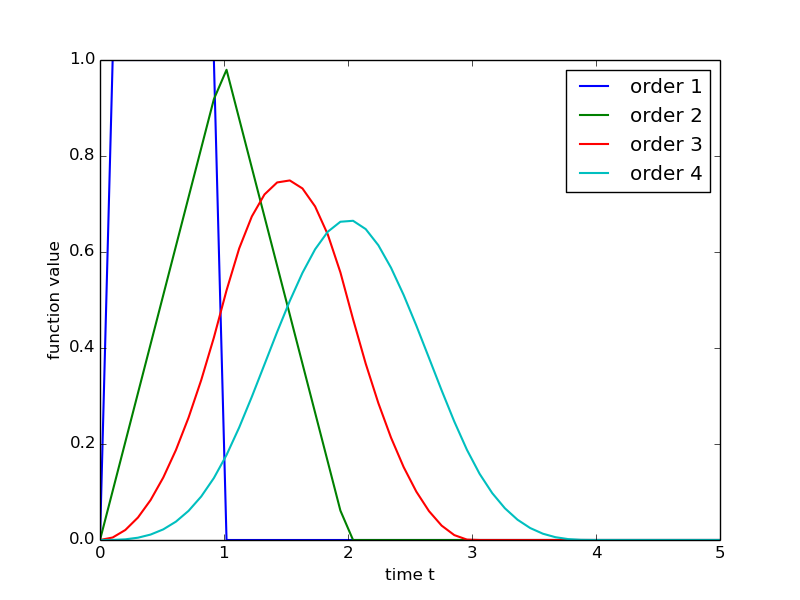
\includegraphics[scale=0.7]{Task_5_1.png}
	\caption{Basis splines of order 1 to 4 in time segment $t_0$ to $t_5$}
	\label{fig:bspline}
\end{figure}
	
	\subsection*{Task 5.2}

	
	\subsection*{Task 5.3}

The Lagrange basis polynomials for l = 3 are calculated as:

\begin{align*}
	L_i(x) = \frac{(x-x_0)(x-x_1)(x-x_2)(x-x_3)}{(x_i-x_0)(x_i-x_1)(x_i-x_2)(x_i-x_3)}
\end{align*}

With our data points

\begin{align*}
x_0 &= 0, y_0 = 1\\
x_1 &= 1, y_1 = 3\\
x_2 &= 3, y_2 = -2\\
x_3 &= 5, y_3 = 4\
\end{align*}

we receive:

\begin{align*}
L_0(x) &= \frac{(x-1)(x-3)(x-5)}{(0-1)(0-3)(0-5)}
 = \frac{x^3-9x^2+23x-15}{-15}\\
L_1(x) &= \frac{(x-0)(x-3)(x-5)}{(1-0)(1-3)(1-5)}
 = \frac{x^3-8x^2+15x}{8}\\
L_2(x) &= \frac{(x-0)(x-1)(x-5)}{(3-0)(3-1)(3-5)}
 = \frac{x^3-6x^2+5x}{-12}\\
L_3(x) &= \frac{(x-0)(x-1)(x-3)}{(5-0)(5-1)(5-3)}
 = \frac{x^3-4x^2+3x}{40}\\
\end{align*}

The Lagrange polynomial $p_3(x)$ is calculated as:

\begin{align*}
p_3(x) &= \sum_{i=0}^{3}y_iL_i(x) \\
&= \frac{x^3-9x^2+23x-15}{-15}+ 3\cdot \frac{x^3-8x^2+15x}{8} -2\cdot \frac{x^3-6x^2+5x}{-12}+ 4\cdot \frac{x^3-4x^2+3x}{40}\\
&= \frac{23x^3}{40}-\frac{19x^2}{5}+\frac{209x}{40}+1
\end{align*}

Langrange basis polynomials and polynomial are plottet in Figure 2.

\begin{figure}[!h]
	\centering
	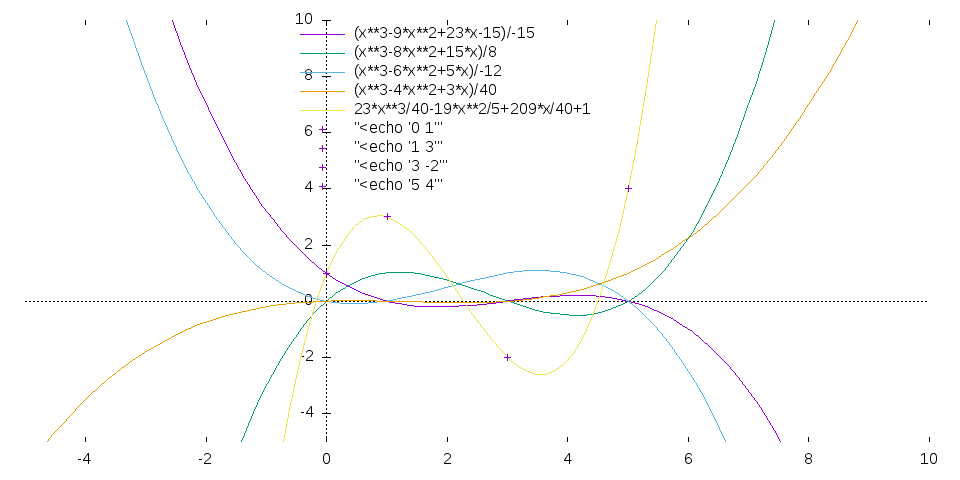
\includegraphics[width= 1\textwidth ]{task52.png}
	\caption{Langrange basis polynomials and polynomial $p_3$.}
\end{figure}
	
	\subsection*{Task 5.4}

The response of a PID-controller is calculated as:

\begin{align*}
	\tau(t) &= k_p \cdot e(t) + k_v \cdot \dot{e}(t) + k_i \int_{t_o}^{t}e(t')dt'
\end{align*}

We consider the error $e(t)$ to be $0$ at the beginning ($t_0$).
Therefore, $e(t), \dot{e}(t)$ and $\int_{t_o}^{t}e(t')dt'$ are $0$ for $t < 0$.

\subsubsection*{5.4.1}

For the heavy-side function as target function the derivative is the Dirac delta function, which is infinite at $t=0$
\begin{align*}
	\delta(t) &= 
	\begin{cases}
		\infty, & t = 0\\
		0, & t \ne 0 
	\end{cases}
\end{align*}
Theoretically the PID-controller is able to set the correct response of infinite at $t=0$ and the error will be $0$ again afterwards.
Overall, the response is then:

\begin{align*}
\tau(t) &= 
\begin{cases}
0, & t < 0\\
\infty, & t = 0\\
0, & t > 0
\end{cases}
\end{align*}

In real applications the correct value won't be reached instantaneous at $t=0$, so that the response will form a flattening curve.\medskip

If the input value is not changed over time and stays at $0$, the target function and the error function are equal: $y(t) = e(t)$.
In that case $e(t) = 1, \dot{e}(t) = 0$ and $\int_{t_o}^{t}e(t')dt' = \int_{t_o}^{t} 1 dt' = t$ for $t > 0$.
The response of the PID-controller is then:
\begin{align*}
\tau(t) &= 
\begin{cases}
0, & t < 0\\
\infty, & t = 0\\
k_p + k_i \cdot t, & t > 0 
\end{cases}
\end{align*}

\begin{figure}[!h]
\centering
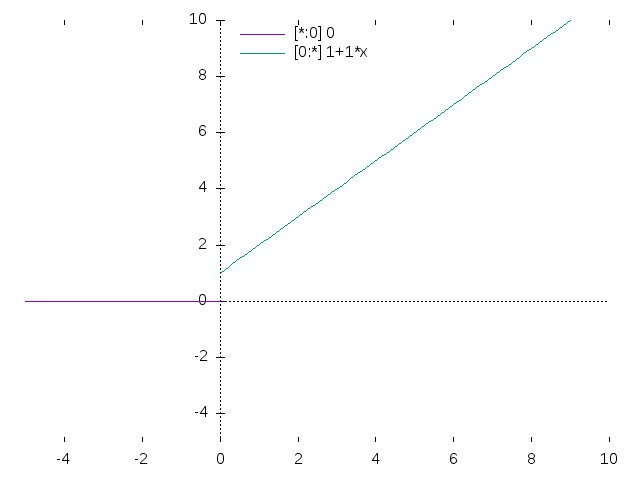
\includegraphics[width= 0.8\textwidth ]{task541.png}
\caption{Output of the PID-controller on the heavy-side function.}
\end{figure}

\subsubsection*{5.4.2}

Considering again that error and target function are equal.\\
The derivative of the error function (ramp function) is the heavy-side function.
And $e(t) = t$ and $\int_{t_o}^{t}e(t')dt' = \int_{t_o}^{t}t'dt' = \frac{1}{2}t^2$ for $t > 0$.\\
The response of the PID-controller is then:
\begin{align*}
\tau(t) &= 
\begin{cases}
0, & t < 0\\
k_p \cdot t + k_v + k_i \cdot \frac{1}{2}t^2, & t \ge 0
\end{cases}
\end{align*}

\begin{figure}[!h]
	\centering
	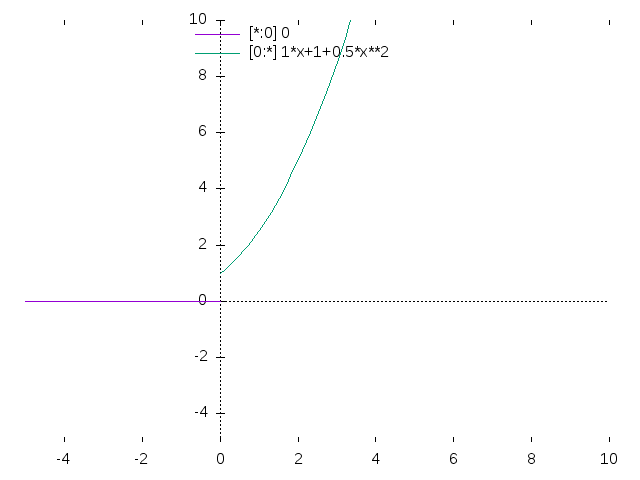
\includegraphics[width= 0.8\textwidth ]{task542.png}
	\caption{Output of the PID-controller on the ramp function.}
\end{figure}





	
\end{document}
